\input{../header}
\usepackage{pgfplots}
\rhead{Your name: \rule{8cm}{0.15mm}}

\begin{document}

\section{Learning target DF1, version 5}

Estimate the value of a derivative using difference quotients, and draw corresponding secant and tangent lines on the graph of a function.

\hrulefill


\everymath{\displaystyle}

Suppose that you know the following values of some function $f(x)$:

\[
\begin{array}{c||r|r|r}
      x  &  1 &  1.5   &  2 \\\hline
    f(x) & -0.8 & -1   & -1.6
\end{array}
\]
\begin{enumerate}[leftmargin=0pt]

\item Plot these points and sketch a plausible graph of $f(x)$.

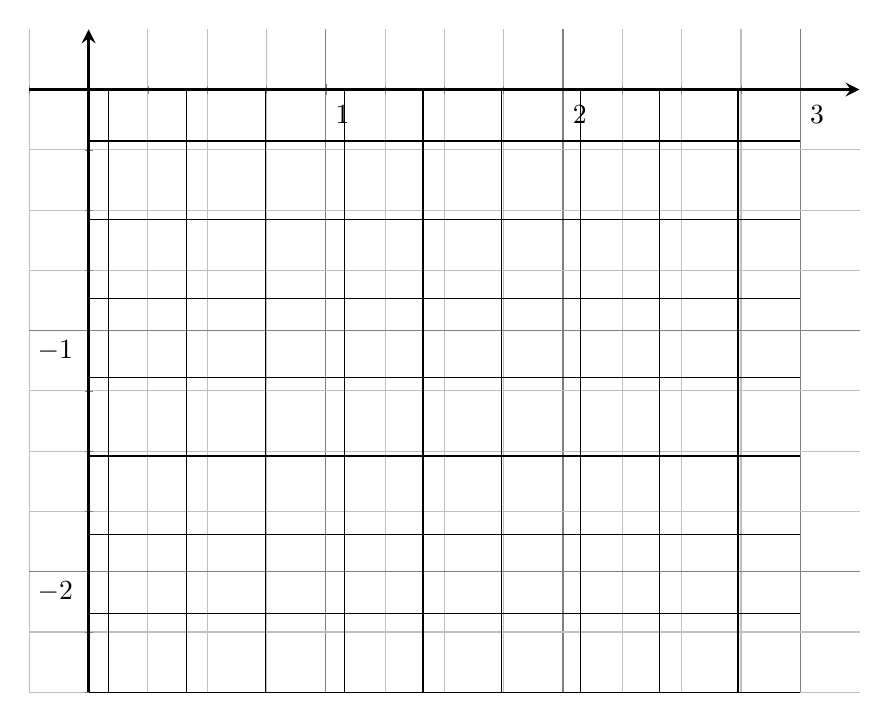
\begin{tikzpicture}
    \begin{axis}[
        width=\textwidth, height=10cm,
        xmin=-0.25, xmax=3.25, ymin=-2.5, ymax=0.25,
        xtick distance = 1, ytick distance = 1,
        minor tick num = 3,
        xticklabel style={anchor=north west},
        yticklabel style={anchor=north east},
        major grid style={thin, black!50},
        grid=both, 
        axis lines=center, axis line style = very thick]
        \draw (0,0) grid (3, -3);
    \end{axis}
\end{tikzpicture}

\item On your graph above, draw a plausible tangent line to the graph of $f(x)$ at $x=1.5$.

\item Use a central difference to estimate $f'(1.5)$. Draw the corresponding secant line on your graph.
\vfill

\item Compute another, different estimate of $f'(1.5)$. Draw the corresponding secant line on your graph.

\vfill

\item Which one of your approximations is the best? How do you know?

\vspace{1cm}

\end{enumerate}

%%%%%%%%%%%%%%%%%%%%%%%%%%%%%%%%%%%%%%%%%%%%%
\pagebreak
%%%%%%%%%%%%%%%%%%%%%%%%%%%%%%%%%%%%%%%%%%%%%

\section{Learning target AD2, version 4}

Part of the graph of this function $f(x)$ has been erased. 
We'll use linear approximation to recover the values.

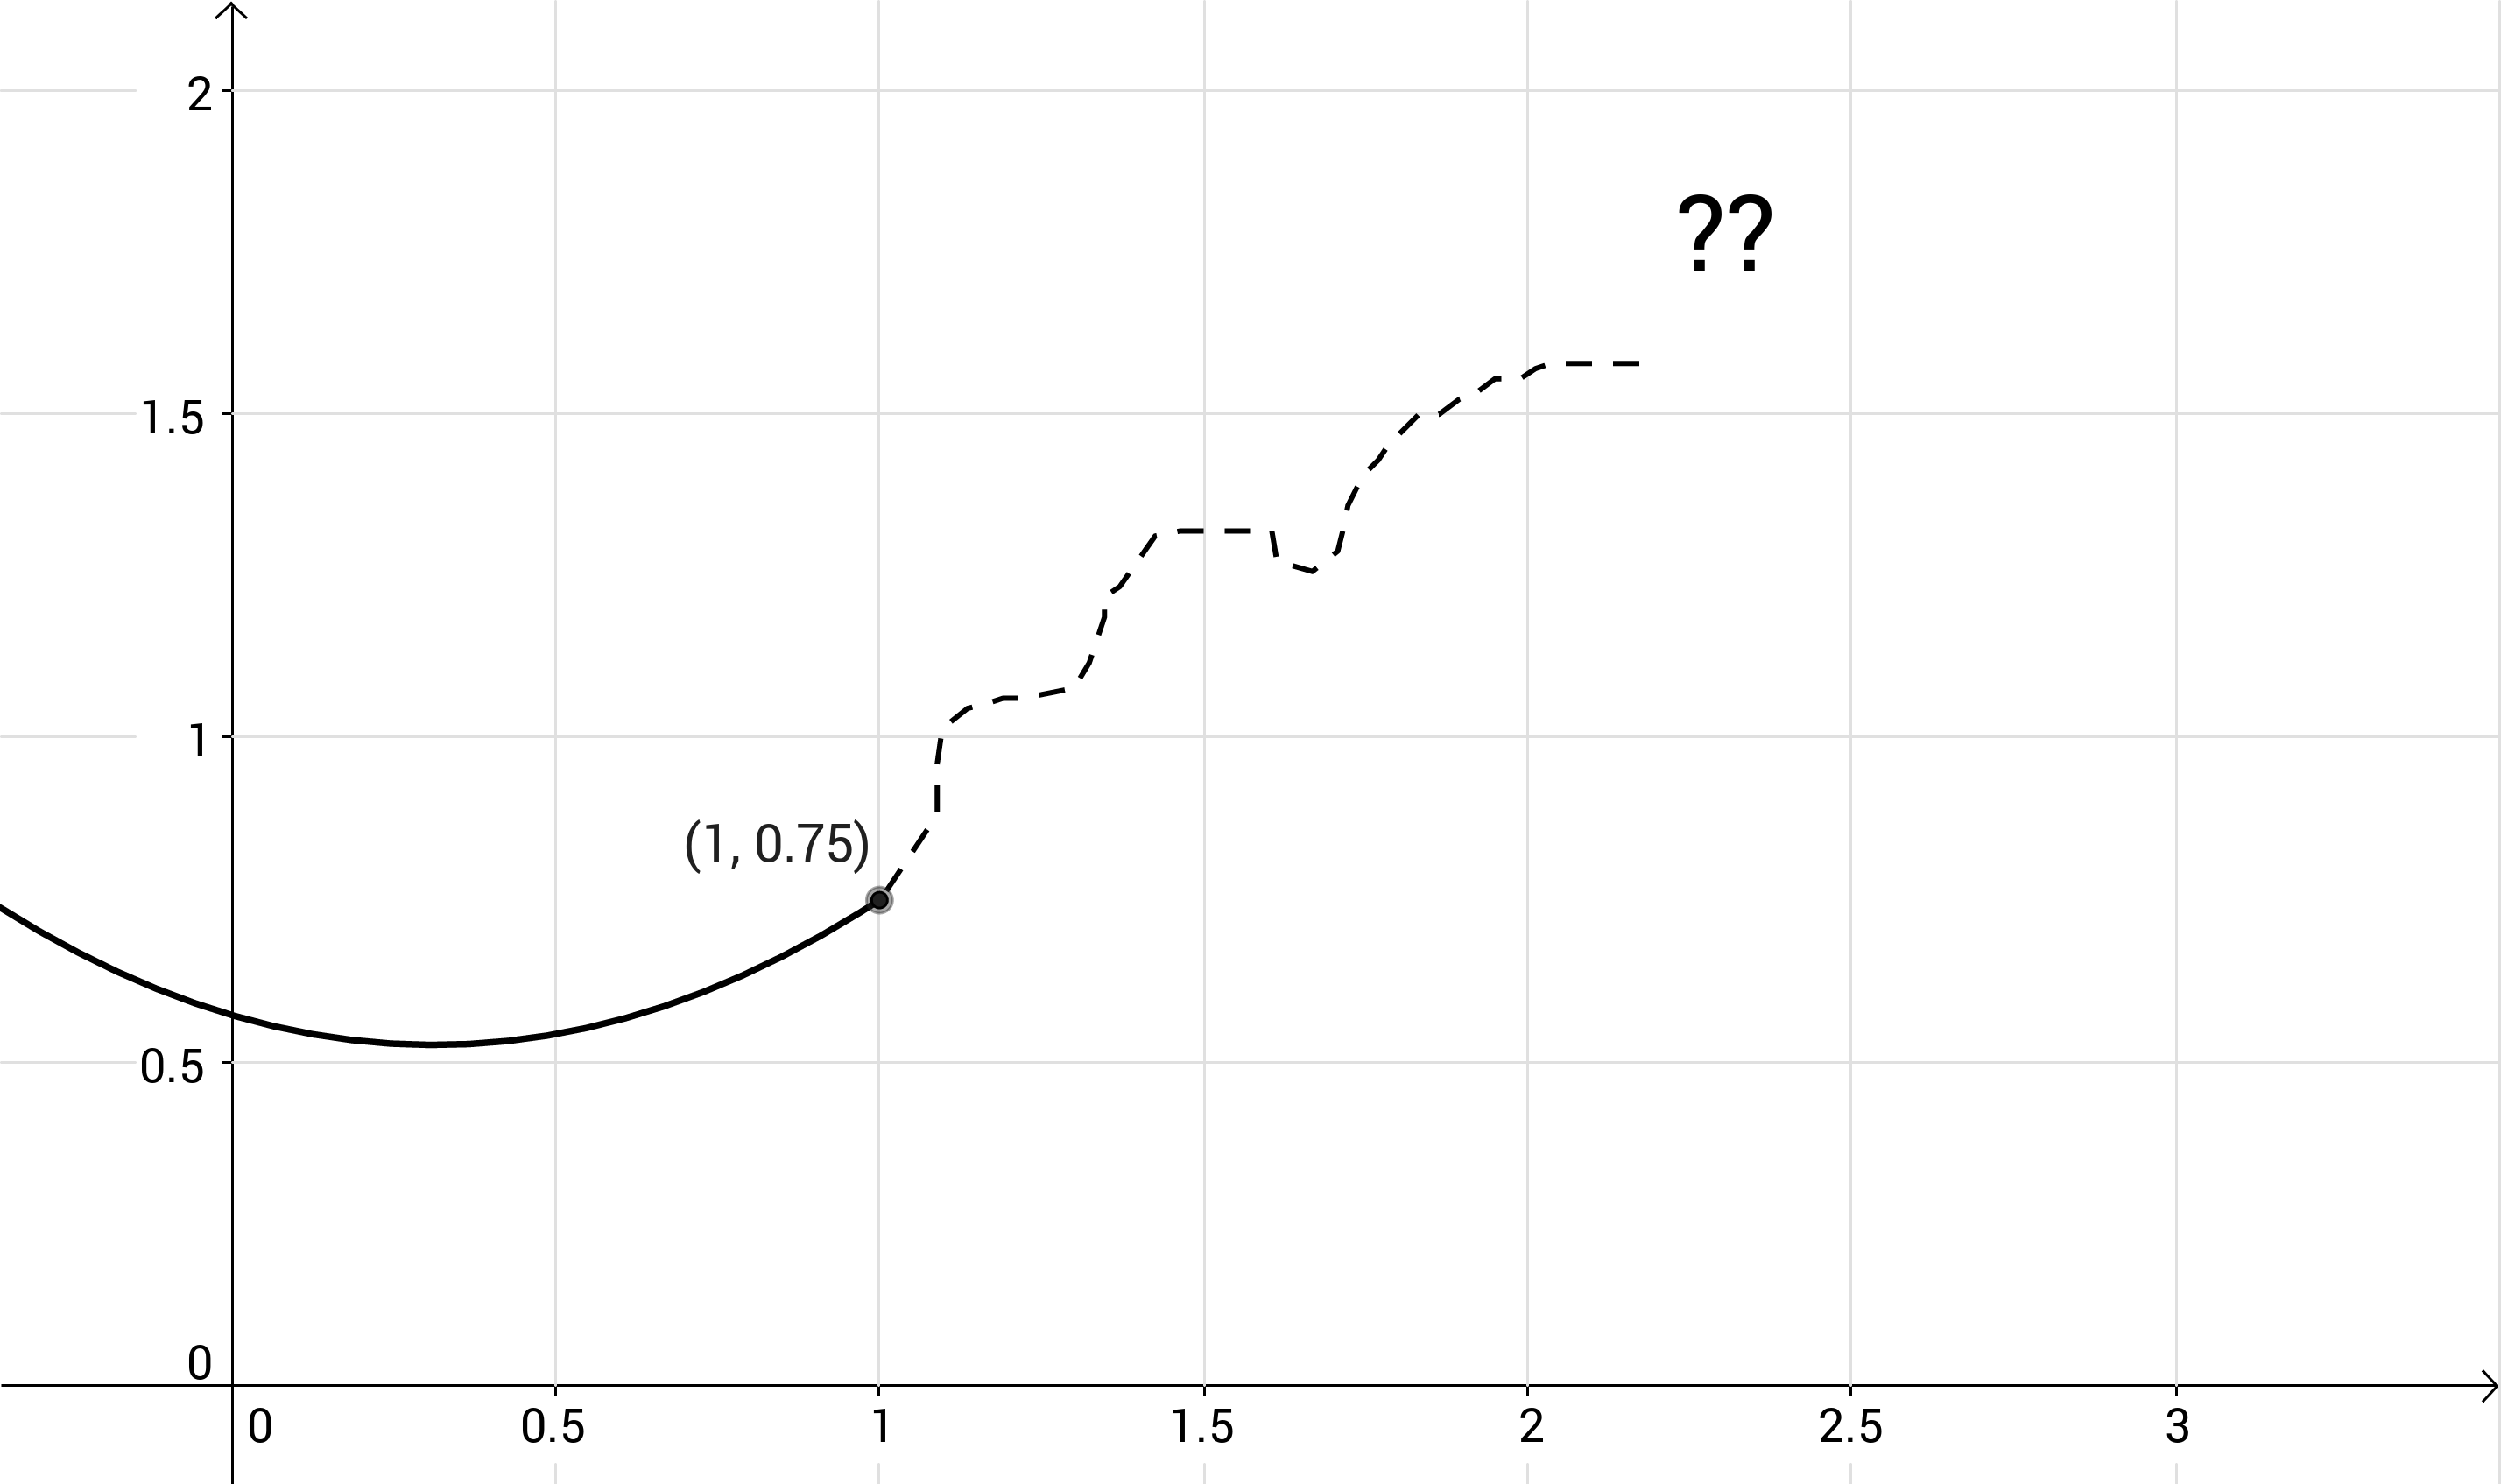
\includegraphics[width=\textwidth]{../images/linapprox.png}

\begin{enumerate}[(a)]
\item Draw the tangent line to this function at $x = 1$.
\item Suppose we know that $f'(1) = 0.65$. Use point-slope form to write down an equation for $L(x)$, the tangent line to this function at $x=1$.
\vfill
\item Use your equation for $L(x)$ to estimate $f(1.4)$.
\vfill
\item Do you think it is more likely that this is an 
overestimate or an underestimate? How come?
\vfill

\end{enumerate}

%%%%%%%%%%%%%%%%%%%%%%%%%%%%%%%%%%%%%%%%%%%%%%%%%%%%%%%%%
\pagebreak
%%%%%%%%%%%%%%%%%%%%%%%%%%%%%%%%%%%%%%%%%%%%%%%%%%%%%%%%%

\section{Learning target DF5, version 4}

Compute derivatives using the Chain Rule.

\hrulefill

Demonstrate and explain how to find the derivative of the following functions. Be sure to write down which derivative rules (chain, product, quotient, sum and difference, etc.) you are using.

\begin{enumerate}
    \item \(g(t)= 3 \, \cos\left(-3 \, t^{2} - 3 \, t + 4\right)\)
    \vfill
    \item \(h(y)= 5 \, \sin\left(y^{7/2}\right)\)
    \vfill
    \item \(k(w)= 5 \, \Big(\sin\left(w\right)\Big)^{7/2}\)
    \vfill
    \item \(f(x)= -{\left(5 \, x + 3 \, e^{x} - 4\right)}^{5}\)
    \vfill
\end{enumerate}

%%%%%%%%%%%%%%%%%%%%%%%%%%%%%%%%%%%%%%%%%%%%%%%%%%%%%%%%%
\pagebreak
%%%%%%%%%%%%%%%%%%%%%%%%%%%%%%%%%%%%%%%%%%%%%%%%%%%%%%%%%

\section{Learning target IN1, version 4}

Use geometric formulas to find definite integrals.

\hrulefill

Here is the graph of a function $N(t)$, which is made up of only straight lines and parts of circles.

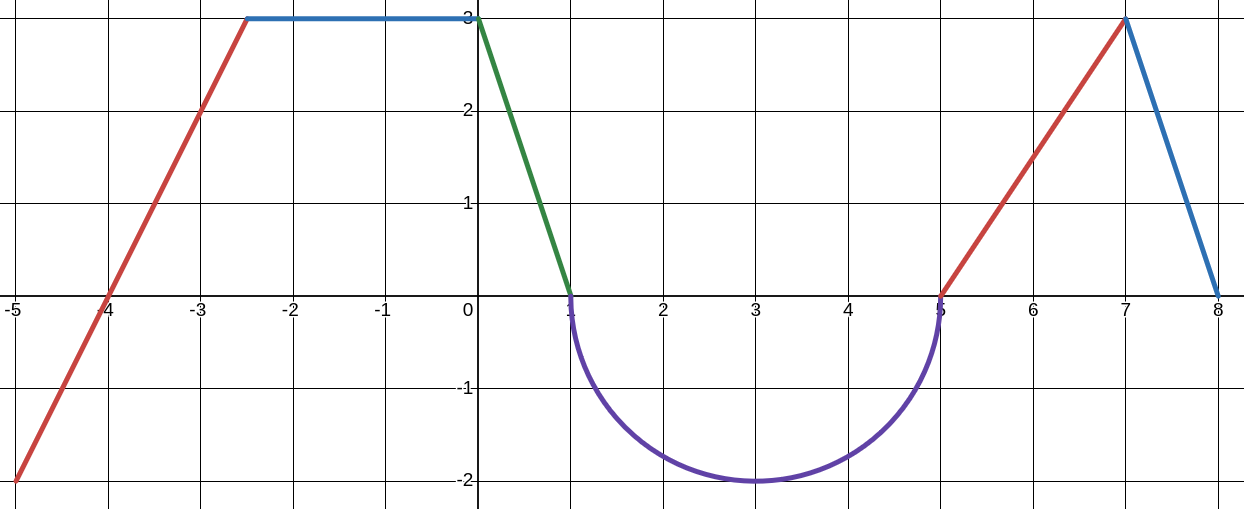
\includegraphics[width=\textwidth]{../images/IN1-v4.png}

Compute each of the following.

\begin{multicols*}{2}
{\everymath{\displaystyle}
\begin{enumerate}[(a)]
    \item $\int_{-5}^{-4} N(t)\ dt$

    \vfill
    \item $\int_{-4}^{-2.5} N(t)\ dt$

    \vfill
    \item $\int_{-2.5}^0 N(t)\ dt$

    \vfill
    \item $\int_0^1 N(t)\ dt$

    \vfill
    \columnbreak
    \item $\int_1^5 N(t)\ dt$

    \vfill
    \item $\int_{5}^7 N(t)\ dt$

    \vfill
    \item $\int_{7}^8 N(t)\ dt$

    \vfill
    \item $\int_{-5}^8 N(t)\ dt$
    

\end{enumerate}
}
\end{multicols*}
%%%%%%%%%%%%%%%%%%%%%%%%%%%%%%%%%%%%%%%%%%%%%%%%%%%%%%%%%
\pagebreak
%%%%%%%%%%%%%%%%%%%%%%%%%%%%%%%%%%%%%%%%%%%%%%%%%%%%%%%%%

\section{Learning target IN2 and INx, version 3}

\iffalse
IN2: Find approximations to definite integrals using variations of Riemann sums.

INx: Correctly interpret the meaning of an area under a curve using the ideas of net change, displacement, etc. Apply the appropriate units to the value.

\hrulefill
\fi

Over the first year of its life, a golden retriever puppy gains weight at a rate of \[p(t) = 4.7 e^{-0.187t} \text{ kilograms per month.}\] 

\fbox{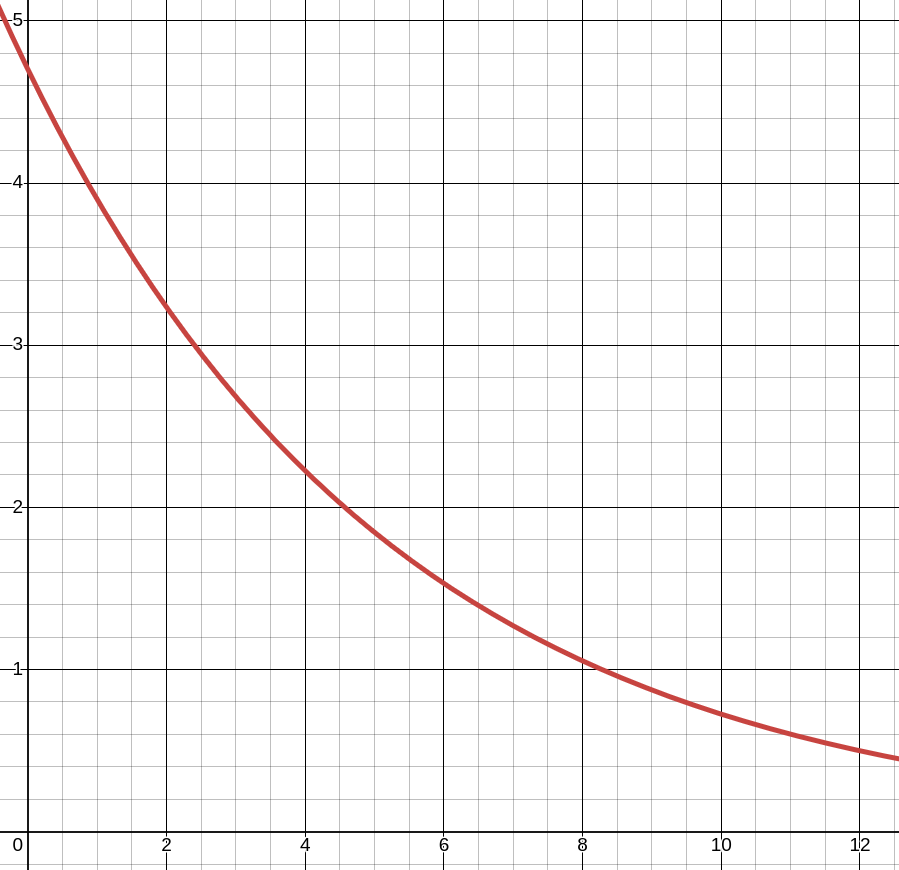
\includegraphics[width=0.5\textwidth]{../images/IN2-v3.png}}
\fbox{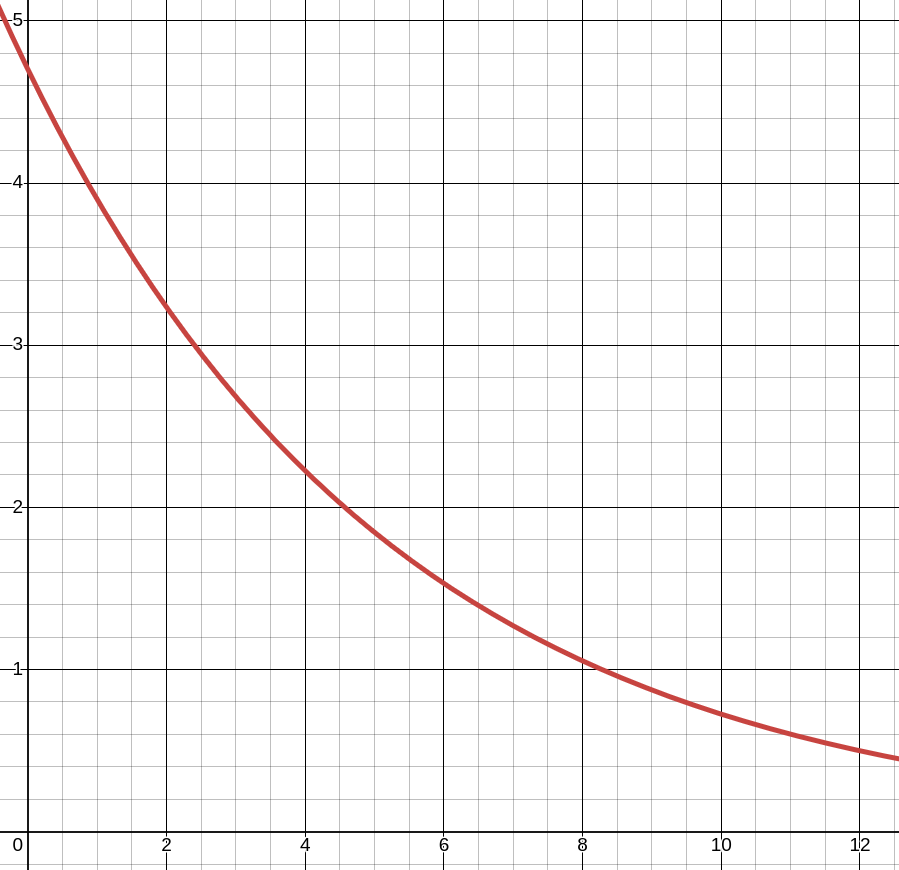
\includegraphics[width=0.5\textwidth]{../images/IN2-v3.png}}
\begin{enumerate}[(a)]
\item On the first graph above, carefully draw the \textit{left} Riemann sum with four rectagles of uniform width. (How wide should each rectangle be?)
\item On the second graph above, carefully draw the \textit{right} Riemann sum with four rectangles.
\item Compute both of these Riemann sums. Show your work for computing the heights of the rectangles. (Hint: lots of your work will overlap!)

\textbf{Include units on every number you write.}
\vfill
\item Give your best guess for $\displaystyle\int_{t=0}^{12} p(t)\, dt$, \textbf{include units}, and explain what this number means about the puppy.
\end{enumerate}

\end{document}